\begin{figure}[ht]
    \centering
    \scalebox{1.2}{

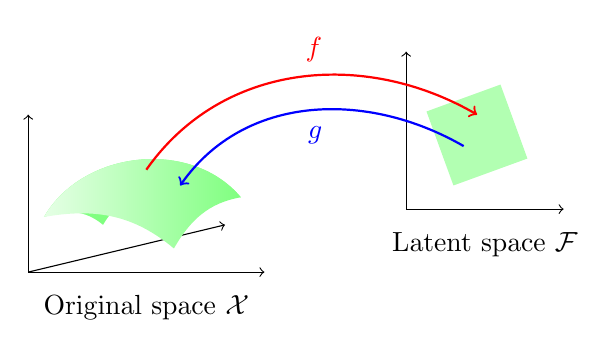
\begin{tikzpicture}
\centering
\draw[->] (0, 0) -- ++(0, 2);
\draw[->] (0, 0) -- ++(2.5, 0.6);
\draw[->] (0, 0) -- ++(3, 0) node[midway, below, yshift=-0.5em]
    {Original space ${\cal X}$};

\draw[fill=green!50, draw=none, shift={(0.2, 0.7)},scale=0.5]
  (0, 0) to[out=20, in=140] (1.5, -0.2) to [out=60, in=160]
  (5, 0.5) to[out=130, in=60]
  cycle;

\shade[thin, left color=green!10, right color=green!50, draw=none,
  shift={(0.2, 0.7)},scale=0.5]
  (0, 0) to[out=10, in=140] (3.3, -0.8) to [out=60, in=190] (5, 0.5)
    to[out=130, in=60] cycle;

  \draw[->] (4.8, 0.8) -- ++(0, 2);
  \draw[->] (4.8, 0.8) -- ++(2, 0) node[midway, below, yshift=-0.5em]
      {Latent space ${\cal F}$};

  \draw[thin, fill=green!30, draw=none, shift={(5.4, 1.1)}, rotate=20]
    (0, 0) -- (1, 0) -- (1, 1) -- (0, 1) -- cycle;

  \draw[thick,->,red]
    (1.5, 1.3) to [out=55, in=150] node[midway, above, xshift=6pt, yshift=2pt]
    {$f$} (5.7, 2);

  \draw[thick,->,blue] (1.5, 1.3) ++(4.03, 0.3) to [out=150, in=55]
    node[midway, below, xshift=2pt, yshift=-2pt] {$g$} ++(-3.6, -0.5);

\end{tikzpicture}}
    
    \caption[Dimensionality reduction and latent space representation \cite{tikz}.]{\small{Dimensionality reduction and latent space representation: Mapping between the original high-dimensional space ${\cal X}$ and the lower-dimensional latent space ${\cal F}$ using functions $f$ and $g$.}}
    \label{fig:manifold}
\end{figure}
